%-------------------------------------------------------------------------------
%                            BAB II
%               TINJAUAN PUSTAKA DAN DASAR TEORI
%-------------------------------------------------------------------------------
\fancyhf{} 
\fancyfoot[C]{\thepage}
\chapter{TINJAUAN KEPUSTAKAAN}

\par Untuk mendukung penelitian ini, maka dalam bab ini akan dikemukakan beberapa rumusan teori pendukung, yang dikutip dari berbagai referensi baik dalam bentuk buku, jurnal, maupun tulisan karya ilmiah lainnya termasuk hasil penelitian sebelumnya yang ada kaitannya dengan penelitian yang dilakukan.                

\section{\uppercase{LOCATION BASED SERVICE (LBS)}}
LBS adalah layanan berupa informasi yang dapat diakses menggunakan \textit{smartphone} melalui jaringan internet dan seluler serta memanfaatkan kemampuan penunjuk lokasi pada \textit{smartphone} \citep{Wardhana2010}. Secara umum sistem LBS terdiri dari 5 komponen, di antaranya perangkat \textit{mobile}, jaringan komunikasi, komponen pelacak posisi untuk mendeteksi lokasi \textit{smartphone}, penyedia layanan dan aplikasi yang memproses permintaan pengguna yang menawarkan data, konten dan layanan yang bisa diminta oleh pengguna \citep{Al-Ammar2014}.

\par Guna meningkatkan akurasi untuk hal LBS, sebuah metode \textit{fingerprinting} telah diterapkan untuk mendeteksi lokasi secara akurat. Metode yang digunakan merupakan salah satu variasi dari RSSI. Selama bertahun-tahun sejumlah alternatif teknologi telah dibuat untuk mendukung teknologi \textit{Location Based Service} untuk \textit{Indoor Positioning} yang paling umum meliputi \textit{Vision}, \textit{Infrared}, \textit{Ultrasound}, \textit{Wireless Local Area Network} (WLAN), \textit{Radio Frequency Identification} (RFID) dan Bluetooth \citep{Olszewski2013}.

\section{\uppercase{INDOOR POSITIONING SYSTEM (IPS)}}
Teknologi berupa layanan untuk menyediakan informasi bagi pengguna berdasarkan lokasi pengguna di suatu ruangan di dalam sebuah gedung, dinamakan IPS \citep{brena2017}. IPS merupakan suatu sistem yang dapat menentukan lokasi \textit{smartphone} yang dimiliki setiap individu di dalam ruangan \citep{suryanto2016}. Banyak penelitian yang telah dilakukan, yaitu implementasi IPS dengan menggunakan pemanfaatan WLAN. Namun, implementasi IPS dengan menggunakan pemanfaatan WLAN memiliki konsumsi daya baterai yang boros pada \textit{smartphone}. Pada akhirnya implementasi IPS diterapkan pada \textit{Bluetooth Low Energy }(BLE) yang memiliki konsumsi daya baterai \textit{smartphone} yang lebih murah. Terdapat tiga pendekatan dalam IPS, yakni berdasarkan jarak (trilaterasi), berdasarkan sudut (triangulasi) dan \textit{fingerprinting}. Metode yang digunakan pada penelitian ini adalah metode \textit{fingerprinting}.
%-----------------------------------------------------------------------------%

%\section{Indoor Localization}
%\textit{Indoor Localization} merupakan. Dalam beberapa tahun terakhir, teknik \textit{Indoor Localization} telah banyak dibahas dan diteliti. Pada dasarnya, biaya yang murah dan akurasi tinggi adalah dua tujuan utama yang terus dikejar para peneliti untuk sistem penentuan posisi dalam ruangan. Sistem penentuan posisi dengan metode trilaterasi menggunakan Wi-Fi dan metode Fingerprinting adalah \textit{hotspot} dalam penelitian penentuan posisi dalam ruangan\citep{}. Beberapa peneliti mendesain sebuah sistem penentuan posisi dalam ruangan dengan menggabungkan Wi-Fi dan teknologi Radio Frequency (RF) lainnya seperti Radio Frequency Identification (RFID) dan Bluetooth Low Energy (BLE) untuk meningkatkan akurasi\citep{}. Metode yang digunakan pada penelitian ini adalah Bluetooth \textit{Fingerprinting} yang merupakan gabungan dari metode trilaterasi.
%-----------------------------------------------------------------------------%

\subsection{Fingerprinting}

\textit{Fingerprinting} merupakan metode yang paling akurat dan populer dalam penggunaannya untuk pelacakan objek pada lingkungan dalam ruangan \citep{Yim2010}. Menurut \cite{Muhammad2018}, \textit{Fingerprinting} adalah teknik untuk menentukan lokasi dengan pemanfaatan \textit{Radio Signal Strength} (RSS) dari suatu \textit{Access Point} (AP). Metode ini memperhitungkan atenuasi karena kekuatan sinyal sering berubah-ubah. Setiap titik referensi dikumpulkan yang mengintegrasikan adanya penghalang antara \textit{receiver} dan \textit{transmitter} \citep{Yudha2018}. \textit{Transmitter} untuk teknologi IPS yang ditujukan untuk WLAN disebut dengan AP, sedangkan \textit{transmitter} untuk teknologi IPS yang ditujukan untuk \textit{Bluetooth Low Energy} (BLE) disebut dengan Beacon. Menurut \cite{Yudha2018}, metode \textit{Fingerprinting} berbasis IPS ini melibatkan 2 tahap yang dapat dilihat pada Gambar \ref{fingerprinting}. 

\fancyhf{} 
\fancyfoot[R]{\thepage}

\begin{figure}[H]
\centering
\shadowbox
{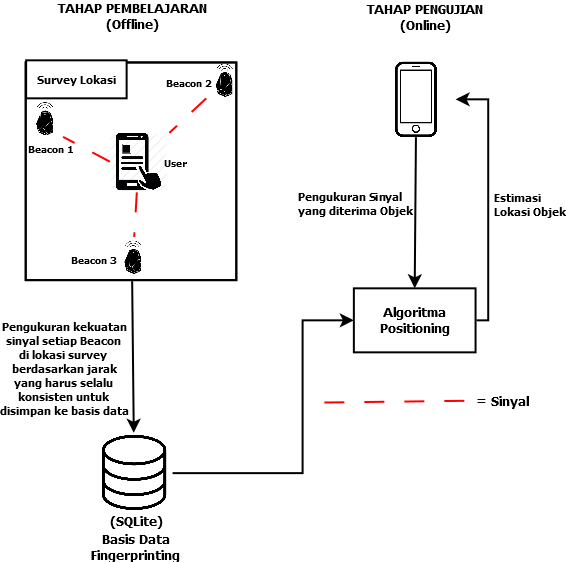
\includegraphics [width = 11cm, height= 9cm]{gambar/fingerprinting}}
\caption{Ilustrasi Metode \textit{Fingerprinting} \citep{Yudha2018}}.
\label{fingerprinting}
\end{figure}

\par Tahap pertama adalah tahap pembelajaran (\textit{offline}), di mana lokasi \textit{Fingerprints} itu sendiri diperoleh dengan cara mengumpulkan RSSI dalam satuan desibel (dBm) yang dipancarkan dari masing-masing AP. Kemudian, gelombang radio akan dipancarkan oleh AP yang diletakkan pada posisi yang telah ditentukan sebelumnya ditangkap oleh \textit{smartphone} dengan kondisi WLAN ataupun Bluetooth dalam keadaan hidup. Selama tahap pembelajaran, lokasi yang tidak diketahui data pembelajarannya kemudian dirujuk sebagai titik referensi estimasi lokasi. 
\newline
\par Tahap kedua adalah tahap pengujian (\textit{online}), di mana keakuratan perkiraan posisi objek sangat bergantung pada jumlah titik referensi yang dikumpulkan dalam data pembelajaran. Selama tahap pengujian, sistem harus memberikan informasi lokasi setiap objek berdasarkan data RSSI yang diamati. Namun, nilai RSSI bisa dipengaruhi oleh keadaan lingkungan sekitar yang dapat mengganggu keakuratannya \citep{Subhan2011}.

\section{\uppercase{RECEIVED SIGNAL STRENGTH INDICATOR (RSSI)}}
\textit{Positioning system} menghasilkan data yang penting untuk menghitung lokasi pengguna. \textit{Time of Arrival} (TOA), \textit{Time Difference of Arrival} (TDOA), \textit{Angle of Arrival} (AOA) dan RSSI adalah metode yang sesuai untuk menghitung data lokasi pengguna untuk kasus \textit{positioning system} \citep{Liu2007}. RSSI menunjukkan kekuatan atau daya yang diterima oleh sinyal \citep{Kajioka2014}. RSSI memperkirakan jarak \textit{node} yang belum diketahui ke referensi node dari beberapa kumpulan unit perhitungan dengan menggunakan atenuasi kekuatan sinyal (\textit{signal strength}) yang dipancarkan dari \textit{transmitter}. Metode ini tepat dilakukan dengan frekuensi sinyal radio \citep{Schneegans2007}.

\par Sebuah nilai RSSI didefinisikan dengan bilangan negatif. Semakin tinggi bilangan negatifnya, maka kekuatan sinyal tersebut tergolong lemah. Namun, jika bilangan nilai RSSI mendekati 0, maka kekuatan sinyal tersebut tergolong kuat. Biasanya, jika suatu objek berada di dekat AP atau \textit{transmitter}, RSSI akan memperoleh nilai yang besar. RSSI dapat digolongkan menjadi 5 kategori kekuatan sinyal seperti terlihat pada Tabel \ref{t_rssi}.

\begin{table}[H]
\centering
\caption{Kekuatan Sinyal RSSI \citep{VerisIndustries2013}}
\label{t_rssi}
\begin{tabular}{|l|l|l|} 
\hline
\textbf{No.} & \textbf{Kekuatan Sinyal} & \textbf{Kualitas Sinyal}  \\ 
\hline
1.           & Kurang dari -40 dB       & Luar Biasa              \\ 
\hline
2.           & -40 dB hingga -55 dB     & Sangat Baik               \\ 
\hline
3.           & -55 dB hingga -70 dB     & Baik                      \\ 
\hline
4.           & -70 dB hingga -80 dB     & Cukup Baik                \\ 
\hline
5.           & Lebih dari -80 dB        & Buruk                     \\
\hline
\end{tabular}
\end{table}

\section{\uppercase{BLUETOOTH LOW ENERGY (BLE)}}
\cite{Keluza2017}, mengemukakan bahwa Bluetooth merupakan alat komunikasi tanpa kabel yang digunakan untuk pertukaran data dalam jarak yang dekat. Bluetooth dikembangkan oleh Ericson di tahun 1994. Kemudian di tahun 1998 Ericson, IBM, Intel, Nokia dan Toshiba membentuk wewenang kekuasaan khusus yang dinamakan dengan Bluetooth Interest Group (SIG). Pertengahan tahun 2010, Bluetooth SIG mengumumkan spesifikasi dari Bluetooth 4.0, yang termasuk di dalamnya meliputi \textit{Bluetooth Classic}, \textit{Bluetooth High Speed} dan BLE. BLE terkadang juga bisa dikatakan sebagai “Bluetooth Pintar”. Meskipun BLE dan \textit{Bluetooth Classic} banyak memiliki kesamaan, BLE sebenarnya memiliki fungsionalitas yang sama sekali berbeda dari \textit{Bluetooth Classic}. 

\par Keunggulan BLE dibandingkan \textit{Bluetooth Classic} adalah konsumsi daya baterai dan energi listrik dari BLE untuk \textit{transfer} data jauh lebih kecil dibandingkan dengan \textit{Bluetooh Classic}, tetapi dengan jangkauan konektivitas dan kapasitas pengiriman data yang sama \citep{bluetoothsig2010}. Karakteristik dari BLE adalah ukurannya yang sangat kecil, biaya murah, serta konsumsi daya rendah yang bisa digunakan sampai beberapa tahun ke depan dengan menggunakan jenis baterai AAA \citep{Keluza2017}. Menurut \cite{Paganini2015}, terdapat beberapa platform yang mendukung BLE dan platfrom tersebut sudah mendukung Bluetooth 4.0. Beberapa platform tersebut adalah sebagai berikut:
\begin {itemize}
\itemsep0em
	\item iOS5+ (lebih dianjurkan iOS7+).
	\item Android 4.3+ (perbaikan \textit{bug} merous di 4.4+).
	\item Apple OS X 10.6+.
	\item Windows 8 (XP, Vista dan Windows 7 hanya mendukung Bluetooth 2.1).
	\item GNU/Linux Vanilla BlueZ 4.93+.
\end{itemize}

\section{\uppercase{BEACON}}
BLE memancarkan sinyal dari alat \textit{transmiter} yang beroperasi menggunakan baterai. Alat \textit{transmiter} tersebut disebut dengan Beacon. Beacon merupakan alat pendeteksi lokasi dengan harga yang terjangkau, ukurannya yang kecil, memiliki daya tahan baterai yang cukup lama, dan tidak membutuhkan energi listrik tambahan. Setiap perangkat \textit{smartphone} dan \textit{tablets} yang mendeteksi sinyal dari Beacon, dapat menghitung jarak dan memperkirakan keberadaan lokasi setiap perangkat sekaligus \citep{Keluza2017}.

\par Kelebihan dari penggunaan Beacon diperkirakan bertahan sampai bertahun-tahun hanya dengan energi baterai, serta tahan terhadap debu dan air sesuai dengan standar IP67, dan memiliki ketelitian sejauh 1-3 meter \citep{Insoft2016}. Teknologi BLE merupakan solusi yang tepat yang digunakan pada Beacon, karena penggunaan dayanya yang murah, BLE juga termasuk sistem yang ramah lingkungan. Penggunaan daya yang murah pada BLE dicapai dengan menjaga waktu proses transmisi data sesingkat mungkin dan mengizinkan perangkat \textit{smartphone} maupun \textit{tablets} berada pada mode tidur saat proses transmisi data \citep{Lindh2015}.

\section{\uppercase{Metode K-NEAREST NEIGHBOR (K-NN)}}
K-NN merupakan salah satu metode klasifikasi yang sederhana. Metode klasifikasi K-NN telah diterapkan sejak tahun 1970 dalam perkiraan statistik dan pengenalan pola \citep{Park2015}. K-NN merupakan salah satu metode klasifikasi menggunakan pendekatan \textit{supervised-learning} sehingga membutuhkan data pembelajaran yang sudah dilabeli \citep{LukitoAntonius2015}. Berdasarkan data pembelajaran tersebut, satu titik dapat diklasifikasikan dengan cara menghitung jarak terdekat dengan \textit{k}-tetangga terdekat di \textit{class} sekitarnya \citep{Kadyan2016}. Setiap data pembelajaran tersebut akan direpresentasikan sebagai sebuah titik pada ruang dimensi \textit{n}. K-NN akan mencari ruang dan pola untuk \textit{k}-tetangga terdekat yang paling dekat dengan data tersebut saat data kelas yang diberikan tidak diketahui \citep{Imandoust2013}.

\begin{figure}[H]
	\centering
	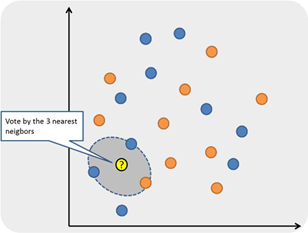
\includegraphics [width = 7cm, height= 5.5cm]{gambar/knn}
	\caption{Ilustrasi Contoh K-NN dengan Nilai \textit{k}=3 \citep{suryanto2016}}.
	\label{knn}
\end{figure}

\par Pada Gambar \ref{knn} terlihat bahwa penentuan kelas dari data baru berdasarkan data pembelajaran dengan ruang 2 dimensi sebagai contoh K-NN dengan nilai \textit{k}=3. Jarak antara data baru dengan data pembelajaran biasanya dihitung berdasarkan fungsi jarak yang umum digunakan yaitu \textit{Euclidean Distance}. Jika terdapat data $P1 = (p_{11}, p_{12},...., p_{1n})$ dan $P2 = (p_{21}, p_{22},...., p_{2n})$ dimana $n$ merupakan jumlah Beacon yang digunakan, maka perhitungan jarak dengan rumus \textit{Euclidean Distance} adalah sebagai berikut:
\begin{equation}
d(P1,P2)=\sqrt{\sum_{i=1}^{n}(p_{1i}-p_{2i})^2}
\end{equation}

\par Algoritma K-NN dikatakan sebagai \textit{nearest neighbor} apabila terdapat kasus khusus yaitu di mana klasifikasi diprediksikan berdasarkan data pembelajaran yang paling dekat (dengan kata lain, nilai \textit{k}=1) \citep{sutarti2016}. Nilai \textit{k} yang terbaik untuk algoritma K-NN bergantung pada banyaknya data. Namun, secara umum nilai \textit{k} yang memiliki nilai sebesar 1 atau 2 memberikan hasil yang terbaik. Nilai \textit{k} yang tinggi akan membuat batasan antara setiap klasifikasi menjadi lebih kabur \citep{otsason2005}.

\section{\uppercase{ANDROID}}
Android adalah sistem operasi untuk perangkat \textit{smartphone} berbasis Linux \citep{Safaat2011}. Android menyediakan platform \textit{open source} bagi para \textit{developer} untuk menciptakan aplikasi mereka sendiri untuk digunakan oleh bermacam peranti bergerak. Aplikasi Android di tulis dengan bahasa pemrograman Java. Bagaimanapun juga, tanpa menggunakan standar Java Virtual Machine (JVM) sebuah aplikasi Android tidak akan bisa berjalan. Android SDK menyediakan sebuah \textit{tools} dan API untuk mengembangkan sebuah aplikasi pada platform \citep{Golhar2016}. Menurut \cite{Supardi2011}, ada 4 komponen utama pada aplikasi Android yaitu sebagai berikut:
\begin{enumerate}[1.]
\itemsep0em
\item \emph{Activities}, merupakan komponen untuk menyajikan tampilan aplikasi kepada pengguna (\textit{user interface}).
\item \emph{Service}, merupakan komponen yang tidak memiliki \textit{user interface} atau disebut dengan \textit{layout} pada Android. Namun, \textit{service} ini bekerja dengan cara \textit{background processing}.
\item \emph{Broadcast Receiver}, merupakan komponen yang berfungsi menerima dan bertugas untuk menyampaikan notifikasi.
\item \emph{Content Provider}, merupakan komponen yang menangani data secara spesifik sehingga dapat digunakan oleh aplikasi lain.
\end{enumerate}

\section{\uppercase{ANDROID STUDIO}}
Android Studio merupakan \textit{Integrated Development Environtment} (IDE) untuk pengembangan platform Android. Android Studio dapat digunakan secara gratis di bawah pengawas Apache License 2.0. Android Studio pertama kali diperlihatkan dimulai dari versi 0.1 pada bulan Mei 2013, kemudian memasuki tahap Beta dimulai dari versi 8.0 yang dirilis pada bulan Juni 2014. Pertama kali dibangun secara stabil pada bulan Desember 2014, dimulai dengan versi 1.0 dikembangkan berdasarkan Jet Brains IntelliJ IDEA \textit{software} dan Android Studio didesain untuk \textit{developer} Android \citep{Singh2016}.

\section{\uppercase{WEB SERVICES}}
\textit{Web services} menggambarkan aplikasi yang mengekspos \textit{business logic} sebagai layanan yang menggunakan internet \citep{Mironela2009}. Layanan tersebut dikirim melalui \textit{interface} yang dapat diprogram, sementara fungsionalitasnya dapat dipakai dan dipanggil melalui alamat \textit{Internet Protocol} (IP \textit{address}) \citep{Wagh2012}. \textit{Web services} sering dikategorikan sebagai komponen sistem perangkat lunak yang dirancang untuk mendukung interaksi antar sistem. \textit{Web services} menyediakan informasi atau data kepada sistem lain untuk digunakan sebagai fasilitas yang membuat sistem dapat saling berinteraksi. Biasanya, data yang diberikan oleh \textit{web services} berupa data dalam bentuk format JavaScript Object Notation (JSON) atau eXtensible Markup Language (XML) \citep{Rahman2013}. Situs \textit{web} World Wide Web Consortium (W3C) mendeskripsikan  bahwa \textit{Simple Object Access Protocol} (SOAP), \textit{REpresentatonal State Transfer} (REST) merupakan protokol yang digunakan \textit{web services} untuk berkomunikasi. Penelitian ini akan menggunakan \textit{web services} dengan layanan protokol REST untuk membantu aplikasi absensi perkuliahan berbasis Android berinteraksi dengan \textit{database} yang terdapat di server.

\section{\uppercase{REpPRESENTATIONAL STATE TRANSFER (REST)}}
REST merupakan hubungan antara klien dan server dan bagaimana sebuah data disimpan. Arsitektur REST didasarkan pada gaya arsitektur klien atau server yang dapat dilihat pada Gambar \ref{restful}. \textit{Request} dan \textit{response} dibangun berdasarkan sumber daya pada saat proses transfer \citep{HaliliRamadani2018}. Konsep dari REST adalah perpindahan antar \textit{state}, dapat dicontohkan seperti sebuah browser yang melakukan permintaan terhadap sebuah halaman situs, maka server akan mengirimkan \textit{state} dari halaman situs tersebut ke browser \citep{Rahman2013}.
\begin{figure}[H]
	\centering
	\shadowbox
	{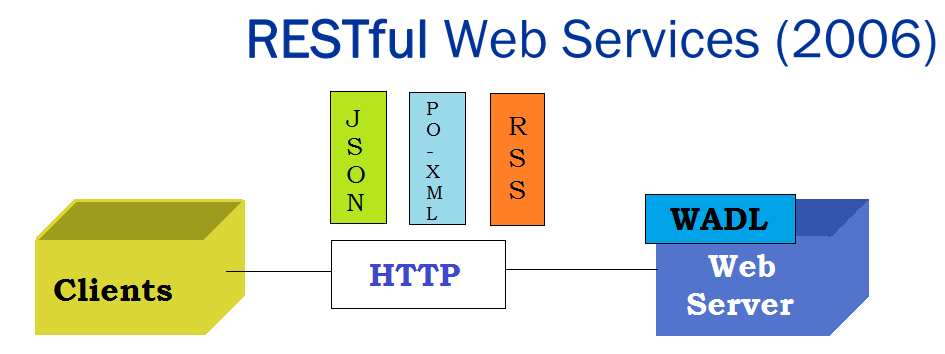
\includegraphics [width = 11cm, height= 3cm]{gambar/restful}}
	\caption
	{Ilustrasi Arsitektur RESTful dan Komunikasi Antara Klien dan Server \citep{HaliliRamadani2018}}.
	\label{restful}
\end{figure}
\par Navigasi REST dilakukan melalui HTTP untuk melakukan aktivitas tertentu, seolah-olah terjadi perpindahan \textit{state} antara satu halaman dengan halaman lainnya \citep{Rahman2013}. Sebuah aplikasi \textit{web} yang bergantung dengan layanan REST arsitektur disebut dengan RESTful \textit{web services}. RESTful \textit{web services} menggunakan 4 perintah HTTP untuk \textit{create}, \textit{read}, \textit{update} dan \textit{delete} yaitu \textit{GET}, \textit{POST}, \textit{PUT} dan \textit{DELETE} seperti yang terlihat pada Gambar \ref{httprestful} \citep{sinha2014}.
\begin{figure}[H]
	\centering
	\shadowbox
	{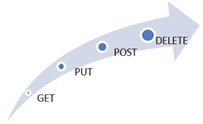
\includegraphics [width = 5cm, height= 3cm]{gambar/httprestful}}
	\caption{Perintah HTTP RESTful \citep{sinha2014}}.
	\label{httprestful}
\end{figure}

\section{\uppercase{SCRUM}}
\textit{Scrum} pada dasarnya didasari oleh proses model \textit{Incremental} yang merupakan salah satu model pengembangan perangkat lunak. Dalam metode \textit{Scrum}, seluruh \textit{development cycle} terbagi menjadi sebuah rangkaian iterasi di mana setiap iterasi tersebut merupakan detak jantung dari \textit{Scrum} itu sendiri yang disebut dengan “\textit{Sprint}”. Pengerjaan \textit{Sprint} memiliki durasi maksimal selama 30 hari. Karena durasi \textit{Sprint} lebih singkat dibandingkan dengan durasi pengembangan produk, maka dalam produk \textit{development cycle} akan ada beberapa \textit{Sprint}, yang artinya pengembangan produk dengan metode \textit{Scrum} dilakukan secara \textit{Iterative} dan \textit{Incremental}. Tahapan-tahapan metode \textit{Scrum} menurut \cite{Schwab2013} adalah sebagai berikut:
\begin {enumerate}[1.]
\item Dimulai dengan mengumpulkan \textit{user requirements}, namun tidak harus semua \textit{requirements} diharapkan harus keluar dari pemikiran \textit{user} di tahap awal proses pengembangan. \textit{User} dapat mengubah pikiran mereka di setiap waktu selama proses pengembangan, \textit{user} dapat menambah fitur-fitur baru, menghapus atau memperbarui beberapa fitur yang telah ada sebelumnya. 
%%%%%%%%%%%%%%%%%%%%%%%%%%%%%%%%%%%%%%%%%%%%%%%%%%%%%%%%%%%%%%%%%%%%%%%%%%%%%%%%%%%%%%%%%%%%%%%%%%%%%%%%%
\item Tahapan selanjutnya adalah memprioritaskan \textit{requirements} dan \textit{Product Backlog}. Sebuah perencanaan yang tepat dalam \textit{Sprint} harus dilakukan sesuai jumlah \textit{Sprint} yang dibutuhkan untuk mengembangkan perangkat lunak, yang terdiri dari durasi \textit{Sprint} tersebut dan \textit{requirements} apa saja yang terdapat di \textit{Product Backlog} yang harus diimplementasikan di setiap \textit{Sprint} (dikenal dengan \textit{Sprint Backlog}). 
%%%%%%%%%%%%%%%%%%%%%%%%%%%%%%%%%%%%%%%%%%%%%%%%%%%%%%%%%%%%%%%%%%%%%%%%%%%%%%%%%%%%%%%%%%%%%%%%%%%%%%%%%
\item \textit{Sprint} diawali dengan \textit{Sprint Planning} dimana \textit{Product Owner}, satu orang yang telah diberikan wewenang dan bertanggung jawab untuk memaksimalkan nilai produk di pasar, bertemu dengan tim \textit{Scrum} (tim dengan jumlah 2-9 orang), kemudian bekerja sama untuk memperkirakan \textit{requirements} dari \textit{Product Backlog} apa saja yang dikerjakan selama satu \textit{Sprint}.
%%%%%%%%%%%%%%%%%%%%%%%%%%%%%%%%%%%%%%%%%%%%%%%%%%%%%%%%%%%%%%%%%%%%%%%%%%%%%%%%%%%%%%%%%%%%%%%%%%%%%%%%% 
\item \textit{Sprint Planning} difasilitasi dengan \textit{Scrum Master}. \textit{Scrum Master} adalah seorang pemimpin yang melayani (\textit{Servant Leader}). \textit{Sprint Planning} memiliki batasan waktu selama 8 jam di dalam sebuah \textit{Sprint} yang berdurasi selama 30 hari. Keluaran dari \textit{Sprint Planning} adalah daftar pekerjaan dari hasil kesepakatan antara \textit{Product Owner} dan tim \textit{Scrum} dimana pekerjaan itu yang akan dikerjakan oleh tim \textit{Scrum} nantinya selama satu \textit{Sprint} beserta \textit{Sprint Goal} yang dinamakan dengan \textit{Sprint Backlog}. 
%%%%%%%%%%%%%%%%%%%%%%%%%%%%%%%%%%%%%%%%%%%%%%%%%%%%%%%%%%%%%%%%%%%%%%%%%%%%%%%%%%%%%%%%%%%%%%%%%%%%%%%%%
\item Setelah \textit{Sprint Planning} berakhir, tim \textit{Scrum} akan mengambil \textit{Sprint Backlog} untuk diri mereka masing-masing dan mengerjakan \textit{Sprint Backlog} setiap hari hingga akhir \textit{Sprint} tanpa campur tangan dari pihak manapun. \textit{Daily Scrum} akan dikerjakan oleh tim \textit{Scrum} yang tidak lebih dari 15 menit untuk menentukan apa saja yang akan mereka kerjakan selama 24 jam ke depan berdasarkan perkembangan 24 jam terakhir, serta menyampaikan permasalahan yang menghambat mereka untuk bisa mencapai \textit{Sprint Goal}. Tim \textit{Scrum} akan melakukan perbaikan-perbaikan item dari \textit{Product Backlog} pada \textit{Sprint} yang akan datang selama proses pengembangan berlangsung, dengan tujuan membuat \textit{Sprint Planning} menjadi lebih efektif.
%%%%%%%%%%%%%%%%%%%%%%%%%%%%%%%%%%%%%%%%%%%%%%%%%%%%%%%%%%%%%%%%%%%%%%%%%%%%%%%%%%%%%%%%%%%%%%%%%%%%%%%%%
\item Di akhir \textit{Sprint} saat acara \textit{Sprint Review}, \textit{Product Owner} akan mempresentasikan hasil pekerjaan tim \textit{Scrum} selama satu \textit{Sprint} dan juga menjelaskan apa saja pencapaian tim \textit{Scrum} menuju \textit{Sprint Goal} di dalam \textit{Sprint} tersebut kepada para pemegang kepentingan (\textit{stakeholder}) agar mendapatkan \textit{feedback}. \textit{Feedback} ini akan dimasukkan ke dalam \textit{Product Backlog} agar meningkatkan nilai dari sebuah produk. \textit{Sprint Review} memiliki batasan waktu tidak lebih dari 4 jam untuk \textit{Sprint} yang memiliki durasi selama 30 hari.
%%%%%%%%%%%%%%%%%%%%%%%%%%%%%%%%%%%%%%%%%%%%%%%%%%%%%%%%%%%%%%%%%%%%%%%%%%%%%%%%%%%%%%%%%%%%%%%%%%%%%%%%%
\item Setelah \textit{Sprint Review}, \textit{Scrum Master} memfasilitasi acara yang bernama \textit{Sprint Retrospectives} agar tim \textit{Scrum}, \textit{Product Owner} bekerja sama menentukan apa saja peningkatan yang akan mereka implementasikan di \textit{Sprint} berikutnya. \textit{Scrum Master} yang efektif, akan kreatif dalam memfasilitasi \textit{Sprint Retrospectives}, akan masuk ke dalam \textit{Sprint Backlog} untuk menuju \textit{Sprint} berikutnya. \textit{Definition of Done} adalah salah satu hal yang ditekankan oleh tim \textit{Scrum} pada saat \textit{Sprint Retrospectives}.
%%%%%%%%%%%%%%%%%%%%%%%%%%%%%%%%%%%%%%%%%%%%%%%%%%%%%%%%%%%%%%%%%%%%%%%%%%%%%%%%%%%%%%%%%%%%%%%%%%%%%%%%%
\item \textit{Sprint Retrospectives} merupakan acara yang paling penting dalam \textit{Scrum} dikarenakan sifatnya yang menekankan \textit{continuous learning} yang dapat meningkatkan tingkat \textit{agility} perusahaan. \textit{Sprint Review} memiliki batasan waktu tidak lebih dari 3 jam untuk \textit{Sprint} yang memiliki durasi selama 30 hari. Setelah \textit{Sprint Retrospectives} berakhir, maka \textit{Sprint} berikutnya akan langsung dilakukan tanpa ada jeda antar \textit{Sprint}. Pada setiap \textit{Sprint}, \textit{Product Owner} akan memastikan agar produk dapat mencapai nilai setinggi mungkin saat pengembangan produk diakhiri. \textit{Product Owner}, \textit{Scrum Master} dan tim \textit{Scrum} memegang komitmen, keberanian, saling menghargai satu sama lain, keterbukaan dan fokus. Ilustrasi tahapan-tahapan metode Scrum dapat dilihat pada Gambar \ref{scrum} dibawah ini.
\end{enumerate} 

\vspace{0,2cm}
\begin{figure}[H]
	\centering
	\shadowbox
	{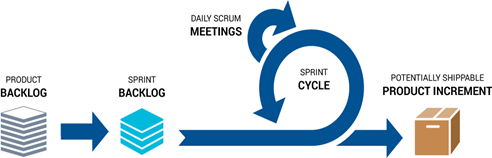
\includegraphics [width = 11cm, height= 3.5cm]{gambar/scrum}}
	\caption{Ilustrasi Metode Pengembangan Menggunakan \textit{Scrum} \citep{Schwab2013}}.
	\label{scrum}
\end{figure}


\section{\uppercase{BLACK BOX TESTING}}
\textit{Black box testing} merupakan pengujian yang hanya dilakukan dengan mengeksekusi dan menjalankan aplikasi itu sendiri untuk mengamati apakah prosesnya sesuai dengan bisnis yang diinginkan \citep{Alfatta2007}. \textit{Black box testing} berfokus pada spesifikasi fungsionalitas perangkat lunak. \textit{Black box testing} menurut \citep{Mustaqbal2015} cenderung menemukan hal-hal berikut:
\begin{enumerate}[1.]
\item Fungsi yang tidak benar atau tidak ada.
\item Kesalahan \textit{user interface}.
\item Kesalahan pada struktur data dan akses \textit{database}.
\item Kesalahan performansi.
\item Kesalahan inisialisasi dan terminasi.
\end{enumerate}

\section{\uppercase{USABILITY TESTING}}
\textit{Usability testing} adalah kegiatan pengujian untuk mengumpulkan data mengenai sebuah produk dalam tahap pengembangan. Tujuan utama dari \textit{usability testing} adalah untuk mengumpulkan data kuantitatif dengan mengukur waktu untuk mempelajarinya, performa kecepatan dan tingkat \textit{human error} \citep{Wahl2000}. \textit{Usability testing} ini dilakukan dengan cara mendudukkan pengguna di pusat, kemudian mengambil pelajaran dari sana. Pengujian ini diharapkan akan mendapatkan kekuatan dan kelemahan dari setiap aspek yang ada pada aplikasi itu sendiri. Maka dari itu, perlu adanya dokumentasi pengalaman aktual para calon pengguna aplikasi atau produk saat dievaluasi \citep{Wesfix2017}.

\par Tujuan lain dilakukannya pengujian ini adalah untuk mengumpulkan data kualitatif yang berhubungan dengan kepuasan pengguna dengan produk yang diuji. Data kualitatif tersebut terdiri dari komentar yang dibuat oleh partisipan, jawaban dari kuisioner pertanyaan dan tanggapan dari partisipan saat proses wawancara. \textit{Usability testing} telah terbukti dapat mengurangi waktu tahap pengembangan, mengurangi jumlah \textit{bugs}, dan menghasilkan produk yang lebih berkualitas untuk meningkatkan nilai jual \citep{Wahl2000}.

\subsection{System Usablity Scale (SUS)}
Metode pengujian dengan \textit{usablity testing} yang digunakan pada penelitian ini adalah SUS. Pada tahun 1996, John Broke menerbitkan sebuah makalah tentang “\textit{quick and dirty}” unidimensional \textit{usability scale} yang dinamakan dengan \textit{System Usablity Scale} (SUS). SUS dikembangkan sebagai sebuah tanggapan dengan biaya yang murah dan praktis yang berfungsi untuk analisis kegunaan aplikasi/produk. Metode pengujian SUS merupakan pengujian untuk mendapatkan penilaian subjektif dari sudut pandang pengguna \citep{Brooke1996}.

\par Skala penilaian yang digunakan yaitu skala likert antara 1-5. \cite{Sugiyono2004} mengatakan bahwa skala likert digunakan untuk mengukur pendapat, persepsi dan sikap seseorang atau sekelompok orang tentang fenomena sosial. SUS bertujuan untuk mengetahui penilaian subjektif yang dilakukan dalam pengujian oleh beberapa responden dan meminta pendapat mengenai aplikasi yang akan dibuat pada penelitian ini.
\par Pengujian ini memerlukan kuesioner sebagai teknik pengumpulan informasi pengujian yang didapat dari responden mengenai aplikasi. Kuesioner terdiri dari 10 soal yang terdiri dari pertanyaan positif dan negatif. Pertanyaan positif terdapat pada nomor ganjil (1, 3, 5, 7, 9) dan pertanyaan negatif terdapat pada nomor genap (2, 4, 6, 8, 10). Setiap pertanyaan diberi bobot antara 0-4. Pertanyaan ganjil skor dihitung dengan cara bobot tiap pertanyaan ($x_{i}$) dikurangi 1 (ditulis $x_{i}$ - 1). Sedangkan pertanyaan genap skor dihitung dengan cara 5 dikurangi bobot tiap pertanyaan ($x_{i}$)(ditulis 5 - $x_{i}$) \citep{Ardiansyah2016}. Setiap pertanyaan memiliki 5 pilihan jawaban yang terdiri dari: sangat tidak setuju, tidak setuju, biasa saja, setuju dan sangat setuju.

%\par Rumus menghitung skor pengujian \textit{usability testing} adalah sebagai berikut:
%\begin{equation}
%\overline{x}=\frac{\sum x}{n}
%\end{equation}
%\newline
%Keterangan:\newline
%$\overline{x}$ = skor rata-rata. \newline
%$\sum x$ = jumlah skor SUS. \newline
%$n$ = jumlah responden. 

\subsection{Test Plan}
\textit{Test plan} adalah dokumen yang melibatkan semua anggota tim \textit{developer} untuk melihat apakah fungsionalitas dari produk yang dibuat sudah terpenuhi atau belum. Dengan kata lain, \textit{test plan} disebut sebagai tujuan, perencanaan atau skenario untuk melakukan \textit{testing} yang akan dilakukan baik itu \textit{expert} \textit{user} atau \textit{user} awam. \textit{Test plan} perlu dibuat saat melakukan pengujian karena \textit{test plan} menggambarkan bagaimana cara menguji produk tersebut. \textit{Test plan} memaksa untuk melakukan pengujian secara sistematis \citep{Rubin2008}. Bagian-bagian dari \textit{test plan} menurut \cite{Rubin2008} adalah sebagai berikut:
\begin{itemize}
\item Maksud, tujuan dan sasaran pengujian.
\item Pertanyaan terkait penelitian.
\item Karakteristik partisipan.
\item Metode yang digunakan (\textit{test design}).
\item \textit{List} tugas.
\item Lingkungan pengujian, perlengkapan, dan logistik.
\item Peran moderator pengujian.
\item Data yang dikumpulkan dan langkah-langkah evaluasi.
\item Laporan dan presentasi.
\end{itemize}








%-----------------------------------------------------------------------------%

% Baris ini digunakan untuk membantu dalam melakukan sitasi
% Karena diapit dengan comment, maka baris ini akan diabaikan
% oleh compiler LaTeX.
\begin{comment}
\bibliography{daftar-pustaka}
\end{comment}
